\chapter{Differential expression analysis of AD-risk genes}\label{app_diff_adrisk_others}

This section documents the results from the differential expression and splicing analyses of the other 17 AD-risk genes profiled in the rTg4510 cortex: 
\begin{multicols}{2}
\begin{enumerate}
	\item \textit{Abca1} (\cref{fig:abca1_diff_analysis})
	\item \textit{Abca7} (\cref{fig:abca7_diff_analysis})
	\item \textit{Ank1} (\cref{fig:Ank1_diff_analysis})
	\item \textit{Apoe} (\cref{fig:Apoe_diff_analysis})
	\item \textit{App} (\cref{fig:App_diff_analysis})
	\item \textit{Clu} (\cref{fig:Clu_diff_analysis})
	\item \textit{Fus} (\cref{fig:Fus_diff_analysis})
	\item \textit{Fyn} (\cref{fig:Fyn_diff_analysis})
	\item \textit{Mapt} (\cref{fig:Mapt_diff_analysis})
	\item \textit{Picalm} (\cref{fig:Picalm_diff_analysis})
	\item \textit{Ptk2b} (\cref{fig:Ptk2b_diff_analysis})
	\item \textit{Rhbdf2} (\cref{fig:Rhbdf2_diff_analysis})
	\item \textit{Snca} (\cref{fig:Snca_diff_analysis})
	\item \textit{Sorl1} (\cref{fig:Sorl1_diff_analysis})
	\item \textit{Tardbp} (\cref{fig:Tardbp_diff_analysis})
	\item \textit{Trpa1} (\cref{fig:Trpa1_diff_analysis})
	\item \textit{Vgf} (\cref{fig:Vgf_diff_analysis})
\end{enumerate}
\end{multicols}
Equivalent plots for \textit{Trem2}, \textit{Cd33} and \textit{Bin1} are discussed in detail in \textbf{Chapter 6}, under \cref{trem2_diff}, \cref{cd33_diff} and \cref{bin1_diff}, respectively.

\begin{landscape}
	\begin{figure}[htp]
		\begin{center}
			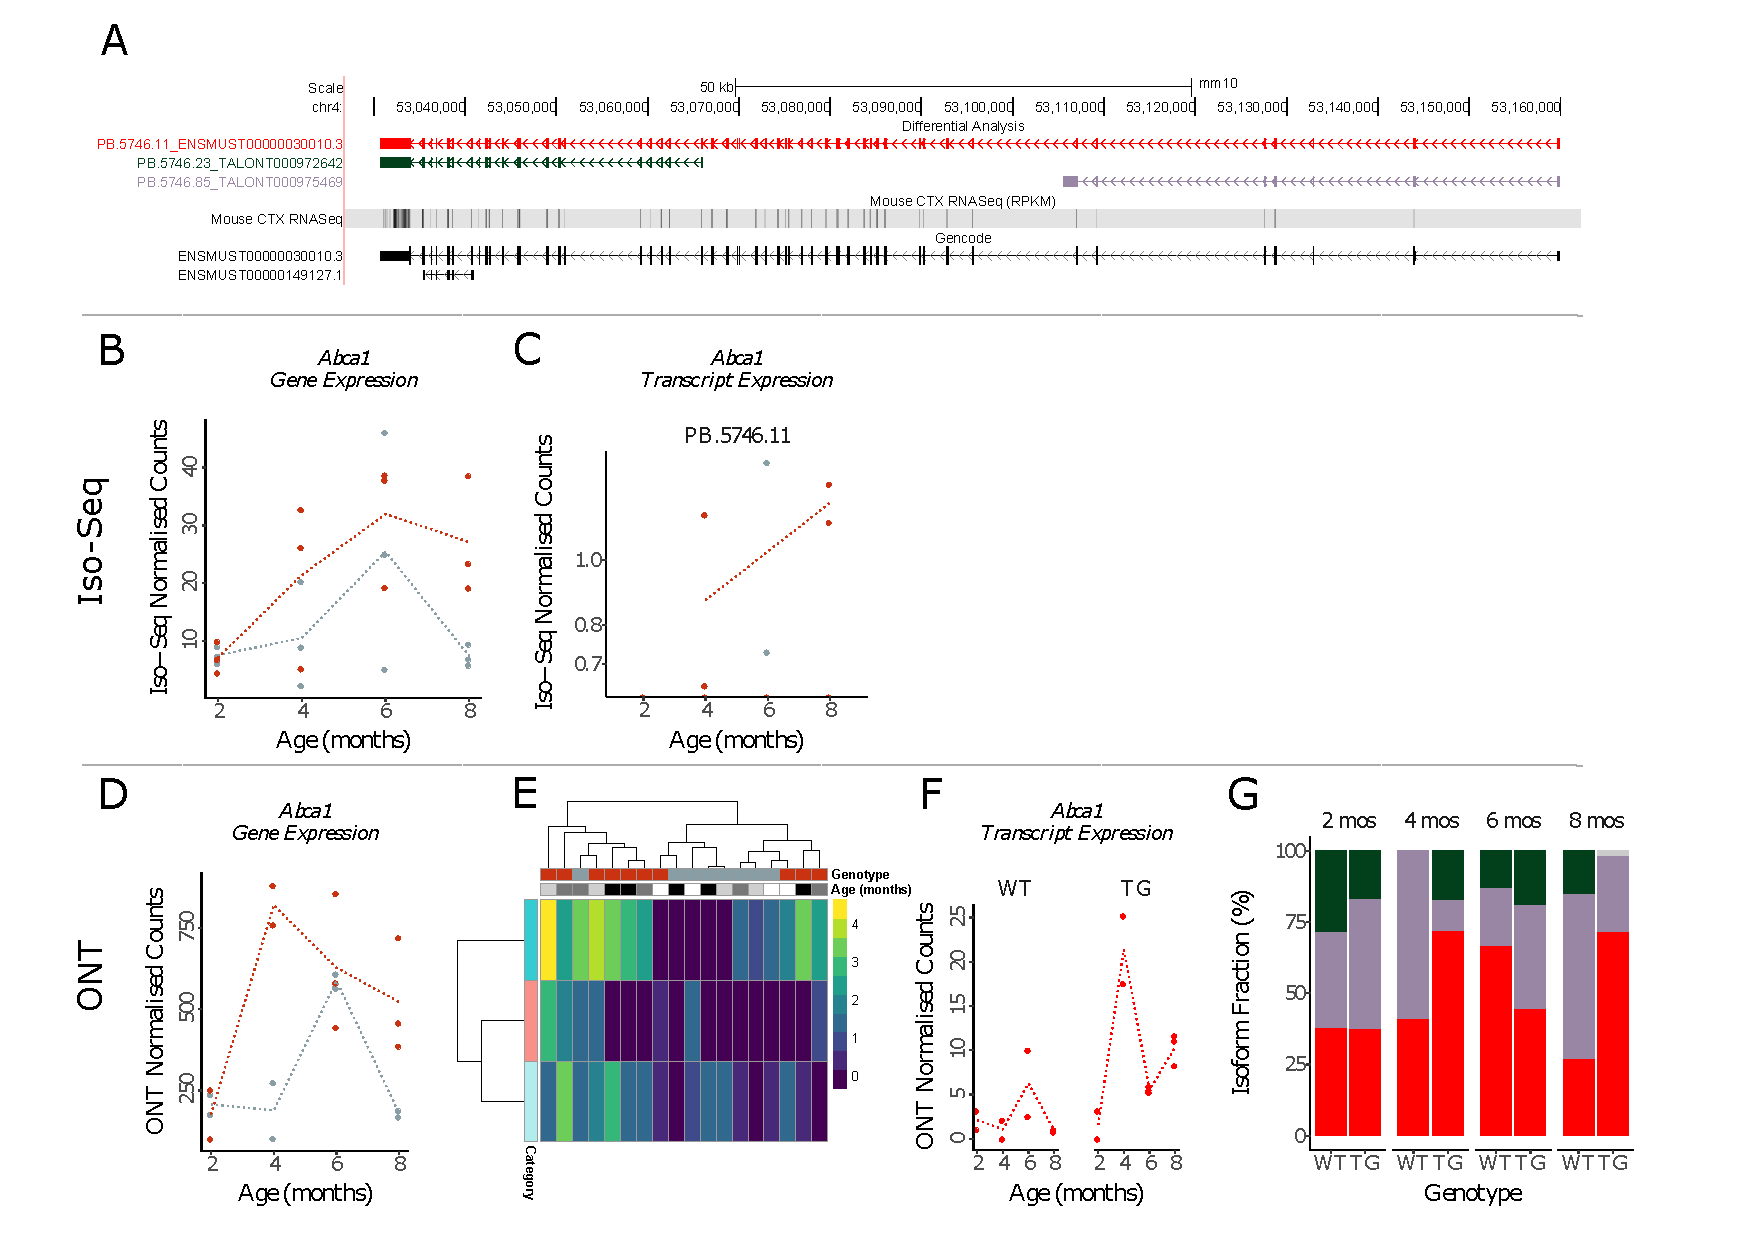
\includegraphics[page=1,trim={0 0.5cm 0 1.5cm},scale =0.85]{Figures/TargetGene_DifferentialAnalysis.pdf}
		\end{center}
		\captionsetup{width=1.5\textwidth}
		\caption[Differential \textit{Abca1} transcript expression and usage]%
		{\textbf{Differential \textit{Abca1} transcript expression and usage}: Shown are plots generated from the differential expression and splicing analyses of \textit{Abca1} in the rTg4510 cortex. \textit{Refer to \cref{fig:cd33_diff_analysis} for the same caption.}}   
		\label{fig:abca1_diff_analysis}
	\end{figure}
\end{landscape}

\begin{landscape}
	\begin{figure}[htp]
		\begin{center}
			\includegraphics[page=2,trim={0 0.5cm 0 1.5cm},scale =0.85]{Figures/TargetGene_DifferentialAnalysis.pdf}
		\end{center}
		\captionsetup{width=1.5\textwidth}
		\caption[Differential \textit{Abca7} transcript expression and usage]%
		{\textbf{Differential \textit{Abca7} transcript expression and usage}: Shown are plots generated from the differential expression and splicing analyses of \textit{Abca7} in the rTg4510 cortex. \textit{Refer to \cref{fig:cd33_diff_analysis} for the same caption.}}   
		\label{fig:abca7_diff_analysis}
	\end{figure}
\end{landscape}

\begin{landscape}
	\begin{figure}[htp]
		\begin{center}
			\includegraphics[page=3,trim={0 0.5cm 0 1.5cm},scale =0.85]{Figures/TargetGene_DifferentialAnalysis.pdf}
		\end{center}
		\captionsetup{width=1.5\textwidth}
		\caption[Differential \textit{Ank1} transcript expression and usage]%
		{\textbf{Differential \textit{Ank1} transcript expression and usage}: Shown are plots generated from the differential expression and splicing analyses of \textit{Ank1} in the rTg4510 cortex. \textit{Refer to \cref{fig:cd33_diff_analysis} for the same caption.}}   
		\label{fig:Ank1_diff_analysis}
	\end{figure}
\end{landscape}

\begin{landscape}
	\begin{figure}[htp]
		\begin{center}
			\includegraphics[page=4,trim={0 0.5cm 0 1.5cm},scale =0.85]{Figures/TargetGene_DifferentialAnalysis.pdf}
		\end{center}
		\captionsetup{width=1.5\textwidth}
		\caption[Differential \textit{Apoe} transcript expression and usage]%
		{\textbf{Differential \textit{Apoe} transcript expression and usage}: Shown are plots generated from the differential expression and splicing analyses of \textit{Apoe} in the rTg4510 cortex. \textit{Refer to \cref{fig:cd33_diff_analysis} for the same caption.}}   
		\label{fig:Apoe_diff_analysis}
	\end{figure}
\end{landscape}

\begin{landscape}
	\begin{figure}[htp]
		\begin{center}
			\includegraphics[page=5,trim={0 0.5cm 0 1.5cm},scale =0.85]{Figures/TargetGene_DifferentialAnalysis.pdf}
		\end{center}
		\captionsetup{width=1.5\textwidth}
		\caption[Differential \textit{App} transcript expression and usage]%
		{\textbf{Differential \textit{App} transcript expression and usage}: Shown are plots generated from the differential expression and splicing analyses of \textit{App} in the rTg4510 cortex. \textit{Refer to \cref{fig:cd33_diff_analysis} for the same caption.}}   
		\label{fig:App_diff_analysis}
	\end{figure}
\end{landscape}

\begin{landscape}
	\begin{figure}[htp]
		\begin{center}
			\includegraphics[page=8,trim={0 0.5cm 0 1.5cm},scale =0.85]{Figures/TargetGene_DifferentialAnalysis.pdf}
		\end{center}
		\captionsetup{width=1.5\textwidth}
		\caption[Differential \textit{Clu} transcript expression and usage]%
		{\textbf{Differential \textit{Clu} transcript expression and usage}: Shown are plots generated from the differential expression and splicing analyses of \textit{Clu} in the rTg4510 cortex. \textit{Refer to \cref{fig:cd33_diff_analysis} for the same caption.}}   
		\label{fig:Clu_diff_analysis}
	\end{figure}
\end{landscape}

\begin{landscape}
	\begin{figure}[htp]
		\begin{center}
			\includegraphics[page=9,trim={0 0.5cm 0 1.5cm},scale =0.85]{Figures/TargetGene_DifferentialAnalysis.pdf}
		\end{center}
		\captionsetup{width=1.5\textwidth}
		\caption[Differential \textit{Fus} transcript expression and usage]%
		{\textbf{Differential \textit{Fus} transcript expression and usage}: Shown are plots generated from the differential expression and splicing analyses of \textit{Fus} in the rTg4510 cortex. \textit{Refer to \cref{fig:cd33_diff_analysis} for the same caption.}}   
		\label{fig:Fus_diff_analysis}
	\end{figure}
\end{landscape}

\begin{landscape}
	\begin{figure}[htp]
		\begin{center}
			\includegraphics[page=10,trim={0 0.5cm 0 1.5cm},scale =0.85]{Figures/TargetGene_DifferentialAnalysis.pdf}
		\end{center}
		\captionsetup{width=1.5\textwidth}
		\caption[Differential \textit{Fyn} transcript expression and usage]%
		{\textbf{Differential \textit{Fyn} transcript expression and usage}: Shown are plots generated from the differential expression and splicing analyses of \textit{Fyn} in the rTg4510 cortex. \textit{Refer to \cref{fig:cd33_diff_analysis} for the same caption.}}   
		\label{fig:Fyn_diff_analysis}
	\end{figure}
\end{landscape}

\begin{landscape}
	\begin{figure}[htp]
		\begin{center}
			\includegraphics[page=11,trim={0 0.5cm 0 1.5cm},scale =0.85]{Figures/TargetGene_DifferentialAnalysis.pdf}
		\end{center}
		\captionsetup{width=1.5\textwidth}
		\caption[Differential \textit{Mapt} transcript expression and usage]%
		{\textbf{Differential \textit{Mapt} transcript expression and usage}: Shown are plots generated from the differential expression and splicing analyses of \textit{Mapt} in the rTg4510 cortex. \textit{Refer to \cref{fig:cd33_diff_analysis} for the same caption.}}   
		\label{fig:Mapt_diff_analysis}
	\end{figure}
\end{landscape}

\begin{landscape}
	\begin{figure}[htp]
		\begin{center}
			\includegraphics[page=12,trim={0 0.5cm 0 1.5cm},scale =0.85]{Figures/TargetGene_DifferentialAnalysis.pdf}
		\end{center}
		\captionsetup{width=1.5\textwidth}
		\caption[Differential \textit{Picalm} transcript expression and usage]%
		{\textbf{Differential \textit{Picalm} transcript expression and usage}: Shown are plots generated from the differential expression and splicing analyses of \textit{Picalm} in the rTg4510 cortex. \textit{Refer to \cref{fig:cd33_diff_analysis} for the same caption.}}   
		\label{fig:Picalm_diff_analysis}
	\end{figure}
\end{landscape}

\begin{landscape}
	\begin{figure}[htp]
		\begin{center}
			\includegraphics[page=13,trim={0 0.5cm 0 1.5cm},scale =0.85]{Figures/TargetGene_DifferentialAnalysis.pdf}
		\end{center}
		\captionsetup{width=1.5\textwidth}
		\caption[Differential \textit{Pt2kb} transcript expression and usage]%
		{\textbf{Differential \textit{Pt2kb} transcript expression and usage}: Shown are plots generated from the differential expression and splicing analyses of \textit{Pt2kb} in the rTg4510 cortex. \textit{Refer to \cref{fig:cd33_diff_analysis} for the same caption.}}   
		\label{fig:Ptk2b_diff_analysis}
	\end{figure}
\end{landscape}

\begin{landscape}
	\begin{figure}[htp]
		\begin{center}
			\includegraphics[page=14,trim={0 0.5cm 0 1.5cm},scale =0.85]{Figures/TargetGene_DifferentialAnalysis.pdf}
		\end{center}
		\captionsetup{width=1.5\textwidth}
		\caption[Differential \textit{Rhbdf2} transcript expression and usage]%
		{\textbf{Differential \textit{Rhbdf2} transcript expression and usage}: Shown are plots generated from the differential expression and splicing analyses of \textit{Rhbdf2} in the rTg4510 cortex. \textit{Refer to \cref{fig:cd33_diff_analysis} for the same caption.}}   
		\label{fig:Rhbdf2_diff_analysis}
	\end{figure}
\end{landscape}

\begin{landscape}
	\begin{figure}[htp]
		\begin{center}
			\includegraphics[page=15,trim={0 0.5cm 0 1.5cm},scale =0.85]{Figures/TargetGene_DifferentialAnalysis.pdf}
		\end{center}
		\captionsetup{width=1.5\textwidth}
		\caption[Differential \textit{Snca} transcript expression and usage]%
		{\textbf{Differential \textit{Snca} transcript expression and usage}: Shown are plots generated from the differential expression and splicing analyses of \textit{Snca} in the rTg4510 cortex. \textit{Refer to \cref{fig:cd33_diff_analysis} for the same caption.}}   
		\label{fig:Snca_diff_analysis}
	\end{figure}
\end{landscape}

\begin{landscape}
	\begin{figure}[htp]
		\begin{center}
			\includegraphics[page=16,trim={0 0.5cm 0 1.5cm},scale =0.85]{Figures/TargetGene_DifferentialAnalysis.pdf}
		\end{center}
		\captionsetup{width=1.5\textwidth}
		\caption[Differential \textit{Sorl1} transcript expression and usage]%
		{\textbf{Differential \textit{Sorl1} transcript expression and usage}: Shown are plots generated from the differential expression and splicing analyses of \textit{Sorl1} in the rTg4510 cortex. \textit{Refer to \cref{fig:cd33_diff_analysis} for the same caption.}}   
		\label{fig:Sorl1_diff_analysis}
	\end{figure}
\end{landscape}

\begin{landscape}
	\begin{figure}[htp]
		\begin{center}
			\includegraphics[page=17,trim={0 0.5cm 0 1.5cm},scale =0.85]{Figures/TargetGene_DifferentialAnalysis.pdf}
		\end{center}
		\captionsetup{width=1.5\textwidth}
		\caption[Differential \textit{Tardbp} transcript expression and usage]%
		{\textbf{Differential \textit{Tardbp} transcript expression and usage}: Shown are plots generated from the differential expression and splicing analyses of \textit{Tardbp} in the rTg4510 cortex. \textit{Refer to \cref{fig:cd33_diff_analysis} for the same caption.}}   
		\label{fig:Tardbp_diff_analysis}
	\end{figure}
\end{landscape}

\begin{landscape}
	\begin{figure}[htp]
		\begin{center}
			\includegraphics[page=19,trim={0 0.5cm 0 1.5cm},scale =0.85]{Figures/TargetGene_DifferentialAnalysis.pdf}
		\end{center}
		\captionsetup{width=1.5\textwidth}
		\caption[Differential \textit{Trpa1} transcript expression and usage]%
		{\textbf{Differential \textit{Trpa1} transcript expression and usage}: Shown are plots generated from the differential expression and splicing analyses of \textit{Trpa1} in the rTg4510 cortex. \textit{Refer to \cref{fig:cd33_diff_analysis} for the same caption.}}   
		\label{fig:Trpa1_diff_analysis}
	\end{figure}
\end{landscape}

\begin{landscape}
	\begin{figure}[htp]
		\begin{center}
			\includegraphics[page=20,trim={0 0.5cm 0 1.5cm},scale =0.85]{Figures/TargetGene_DifferentialAnalysis.pdf}
		\end{center}
		\captionsetup{width=1.5\textwidth}
		\caption[Differential \textit{Vgf} transcript expression and usage]%
		{\textbf{Differential \textit{Vgf} transcript expression and usage}: Shown are plots generated from the differential expression and splicing analyses of \textit{Vgf} in the rTg4510 cortex. \textit{Refer to \cref{fig:cd33_diff_analysis} for the same caption.}}   
		\label{fig:Vgf_diff_analysis}
	\end{figure}
\end{landscape}